%
% This file is part of ICTP RegCM model.
% Copyright (C) 2011 ICTP Trieste
% See the file COPYING for copying conditions.
%

\section{The eforge site}

A new welcoming home for the RegCM Community has been built with the help
of Italian National Research Council CNR Democritos Group on the e-science
Lab E-Forge web site:

\vspace{0.5cm}
\begin{tabular}{|c|}
\hline
{\bf https://eforge.escience-lab.org/gf/project/regcm} \\
\hline
\end{tabular}
\vspace{0.5cm}

\begin{figure}[h!]
\caption{The e-forge site}
\centering
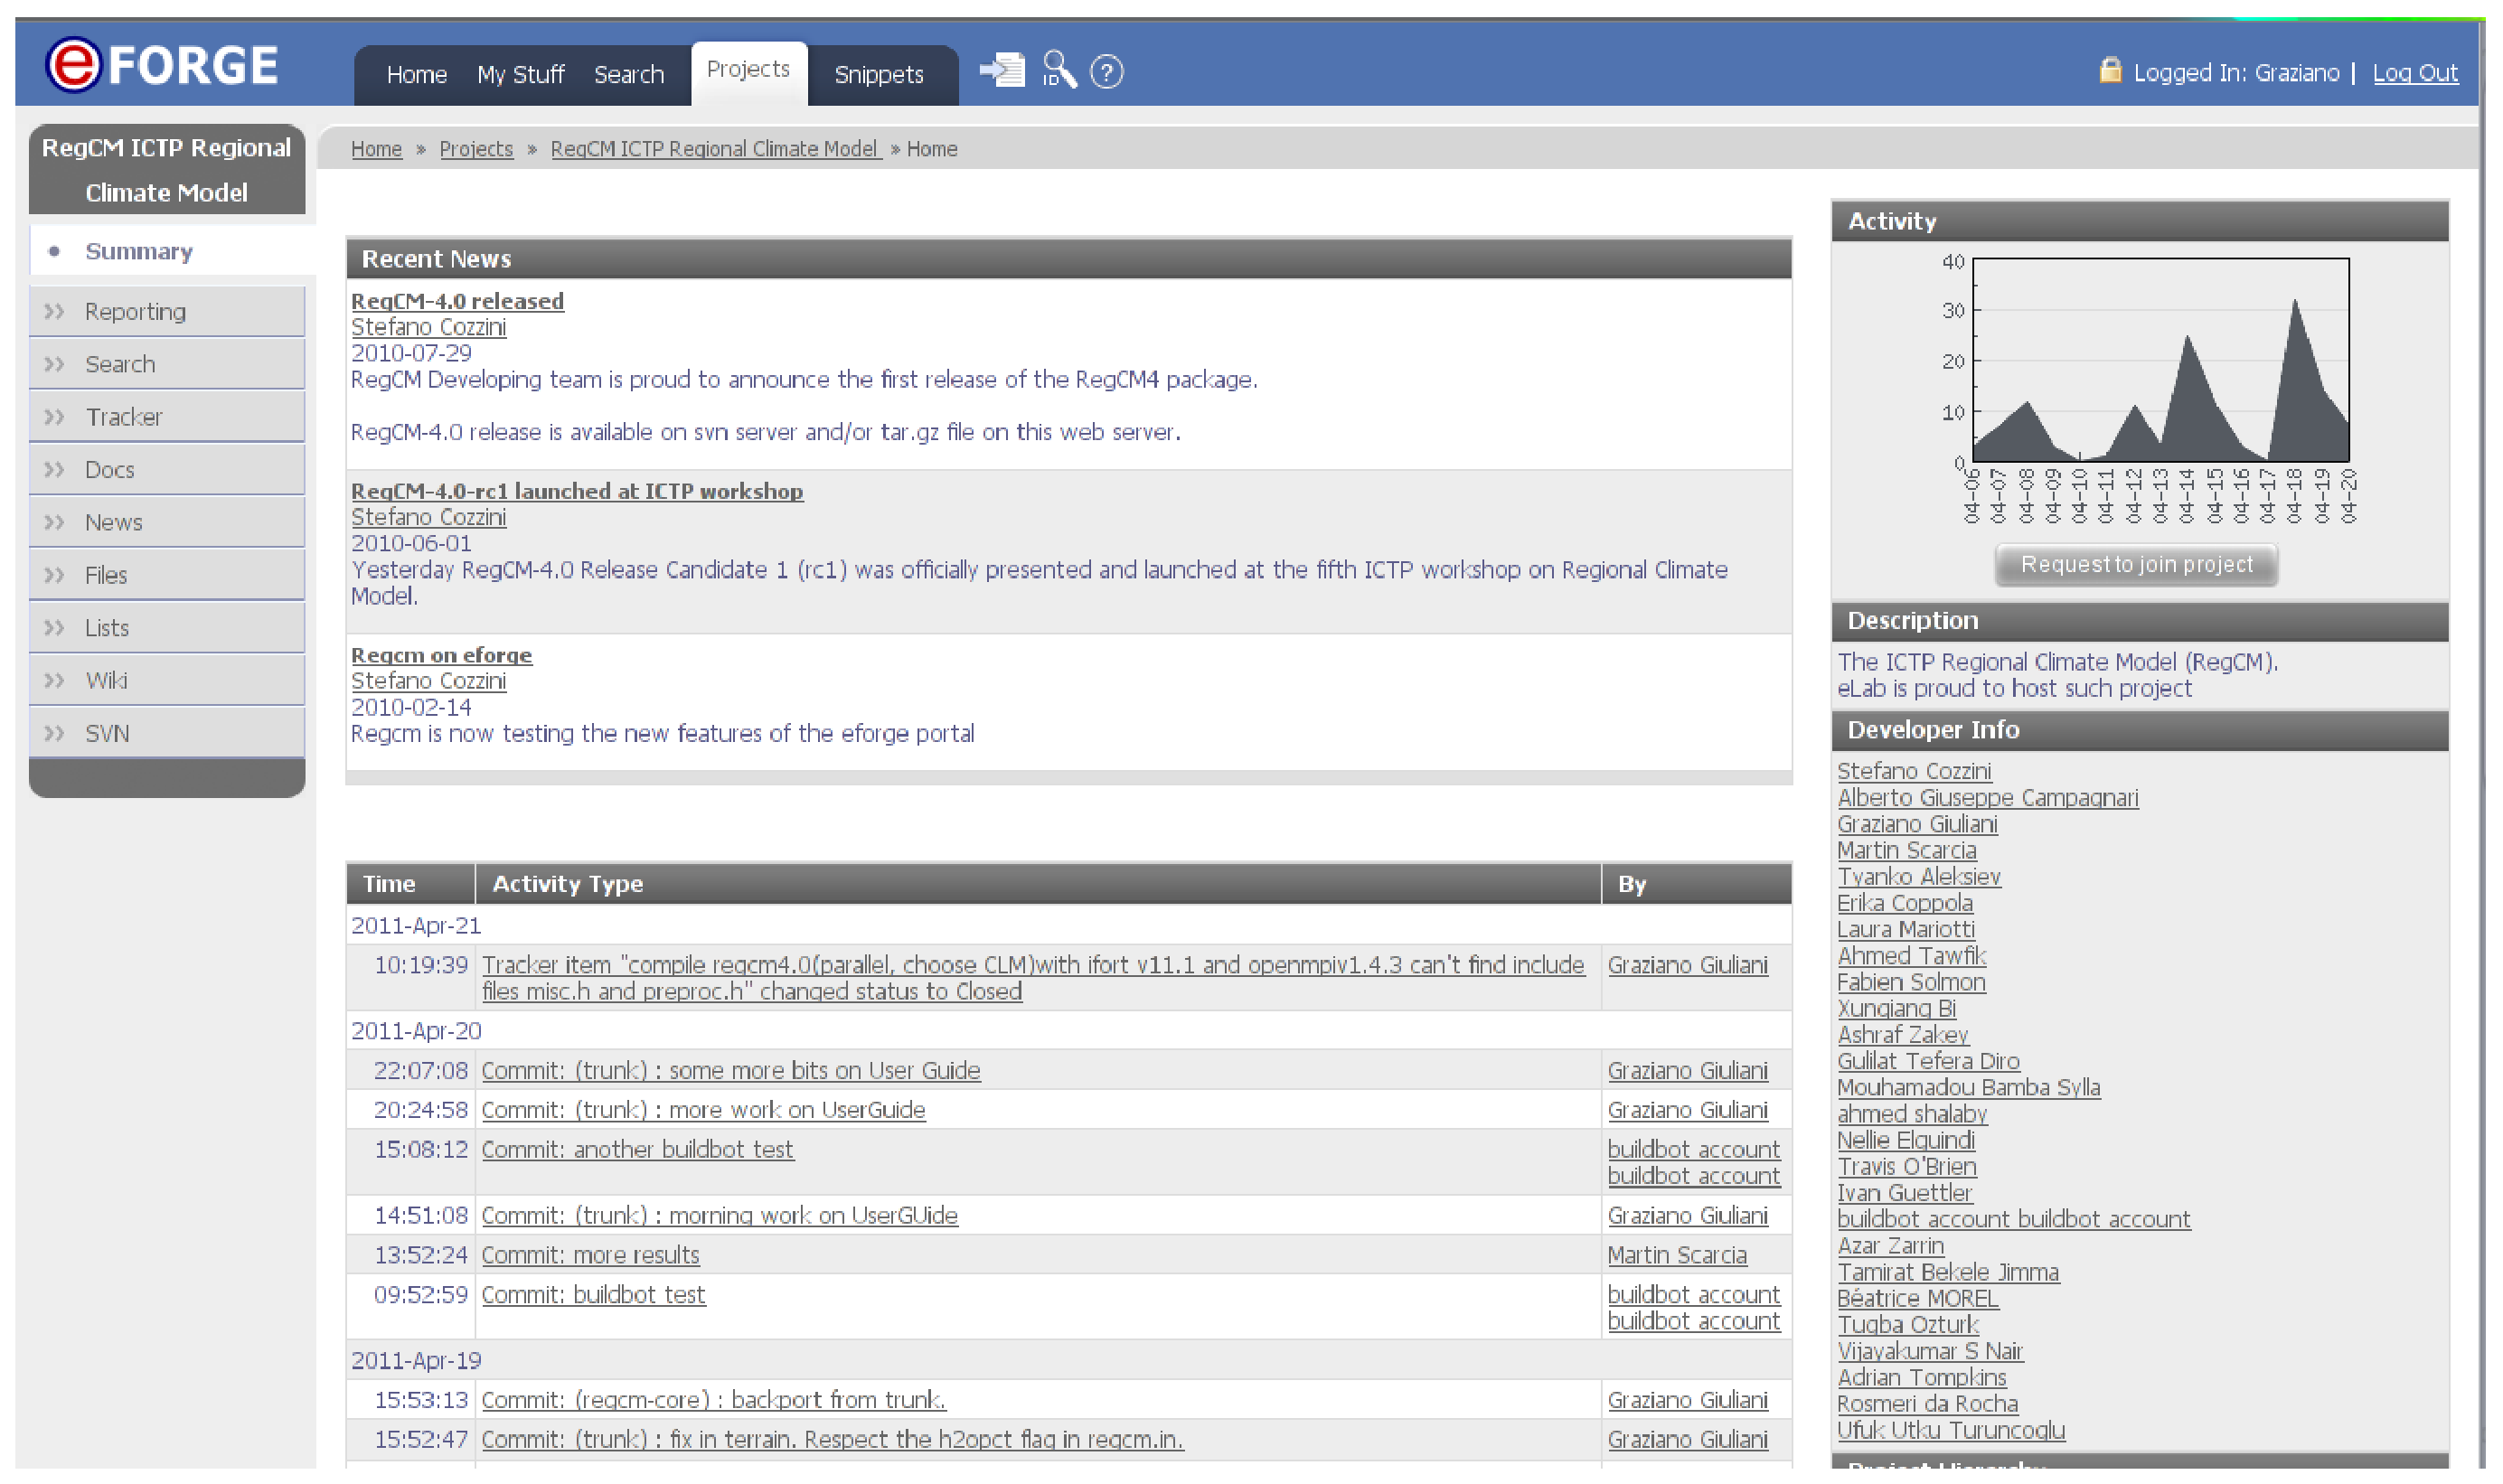
\includegraphics[width=12cm]{e-forge}
\end{figure}

On this site you have access with a simple registration to a friendly
bug tracking system under the {\em tracker} link, allowing the users to
post problems and bugs they discover.

It allows posting also of files to give you the opportunity to provide as
much information as possible about the environment the model is running at
your institution, helping us better understand and solve efficiently your
problems.

Help us grow the model to fit your requirements, giving the broader user
community the benefit of a valuable tool to do better research.

A few general rules, adapted from :
\\
 \\
\verb=http://www.chiark.greenend.org.uk/~sgtatham/bugs.html=

\begin{itemize}
\item The first aim of a bug report is to let us see the failure with our own
eyes. So give us detailed instructions so that we can make it fail for ourself.
\item In case the first aim doesn't succeed, and the programmer can't see it
failing themselves, the second aim of a bug report is to describe what went
wrong. Describe everything in detail. State what you saw, and also state what
you expected to see. Write down the error messages, especially if they have
numbers in.
\item By all means try to diagnose the fault yourself if you think you can, but
if you do, you should still report the symptoms as well.
\item Be ready to provide extra information if the programmer needs it. If they
didn't need it, they wouldn't be asking for it. They aren't being deliberately
awkward. Have version numbers at your fingertips, because they will probably
be needed.
\item Write clearly. Say what you mean, and make sure it can't be
misinterpreted.
\item Above all, be precise.
\end{itemize}

Specific Rules for RegCM package:

\begin{enumerate}
\item Use the tracker system and give us details about which part of the code
failed ( terrain/icbc/regmc/postproc etc)
\item Give us information about compiler you are using
\item Give us information about the version you are using
\item Provide us with your input file so we can test/repeat your problem
\item Be sure to have read the documentation before posting/asking for help
\item Be patient: not  always there is somebody ready to answer your question..
\end{enumerate}

